\documentclass[handout]{beamer}

\usetheme[progressbar=frametitle]{metropolis}
\metroset{block=fill}

\subtitle{NTIN071 Automata and Grammars}
\author{Jakub Bulín (KTIML MFF UK)}

\date{Spring 2025\\ 
    \vspace{1in} 
    \begin{flushleft}
        \it \footnotesize * Adapted from the Czech-lecture slides by Marta Vomlelová with gratitude. The translation, some modifications, and all errors are mine.
    \end{flushleft}
}

%% packages

\usepackage{amsmath}
\usepackage{amssymb}
\usepackage{amsthm}
\usepackage{cancel}
\usepackage{color}
\usepackage{colortbl}
\usepackage{forest}
\usepackage[utf8x]{inputenc}
\usepackage{multicol}
\usepackage{multirow}

%% colors
\definecolor{Gray}{gray}{0.9}

%% TikZ
\usepackage{tikz}
    \usetikzlibrary{
        automata,
        arrows,
        backgrounds,
        decorations.pathmorphing,
        fit,
        positioning,
        shapes,
        shapes.geometric,
        tikzmark
    } 
    \tikzset{>=stealth',shorten >=1pt,auto,node distance=2cm}
    \tikzset{initial text={}}
    \tikzset{elliptic state/.style={draw,ellipse}}

%% amsthm
\theoremstyle{plain}
    \newtheorem*{algorithm}{Algorithm}    
    \newtheorem*{observation}{Observation}
    \newtheorem*{proposition}{Proposition}

\theoremstyle{remark}
    \newtheorem*{exercise}{Exercise}
    \newtheorem*{remark}{Remark}

%% macros
\DeclareMathOperator{\RegE}{RegE}
\DeclareMathOperator{\RL}{RL}

% Just for Lecture 2
\newcommand{\x}{$\times$}
\newcommand{\nx}{\ }



\title{Lecture 11 -- Turing Machines and grammars, Linear bounded automata and context-sensitive grammars, Intro to computability theory}


\begin{document}


\frame{\titlepage}


\begin{frame}{Recap of Lecture 10}
	
    \begin{itemize}        
        \item Turing machine: two-way infinite tape, read, write, move head
        \item Accept iff in a final state; configurations
        \item TMs with output, computing a function
        \item Recursively enumerable vs. recursive languages (always halt).
        \item Construction tricks: 
        \begin{itemize}
            \item storage in state
            \item multiple tracks (on a single tape)
        \end{itemize}
        \item Variants of TMs: 
        \begin{itemize}
            \item multi-tape (independent heads),
            \item nondeterministic (accept iff some choices lead to final state)
        \end{itemize}  
    \end{itemize}
	
\end{frame}


\section{3.3 Turing Machines and grammars}


\begin{frame}{Chomsky hierarchy: Type 0}

    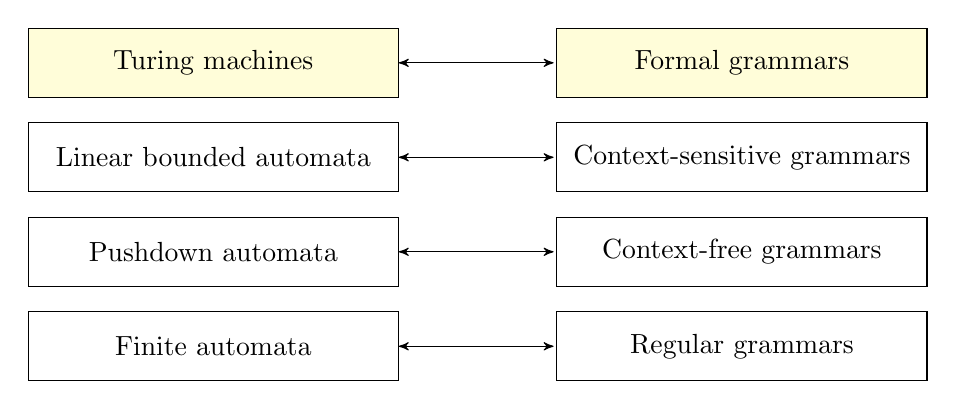
\begin{tikzpicture}[node distance=1.2cm]
        \node[state,rectangle, minimum width =4.7cm][align=center] (fa)      {\alert{Finite automata}};
        \node[state,rectangle, minimum width =4.7cm] (pda) [above of=fa]  {Pushdown automata};
        \node[state,rectangle, minimum width =4.7cm] (la) [above of=pda]  {Linear bounded automata};
        \node[fill=yellow!15!white,state,rectangle, minimum width =4.7cm][align=center] (ts) [above of=la]  {\alert{Turing machines}};
        \node[state,rectangle, minimum width =4.7cm] (rg) [right=2cm of fa]  {Regular grammars};
        \node[state,rectangle, minimum width =4.7cm]  (cfg) [right=2cm of pda]  {\alert{Context-free grammars}};
        \node[state,rectangle, minimum width =4.7cm][align=center]  (cg) [above of=cfg]  {Context-sensitive grammars};
        \node[fill=yellow!15!white,state,rectangle, minimum width =4.7cm] (g0) [above of=cg]  {Formal grammars};
        \path[<->] 
            (fa)  edge node {} (rg)
            (pda)  edge node {} (cfg)
            (la)  edge node {} (cg)
            (ts)  edge node {} (g0)
        ;
    \end{tikzpicture}

    \bigskip

    \begin{theorem}
        A language is recursively enumerable, if and only if it is generated by a Type 0 grammar.
    \end{theorem}
    

\end{frame}


\begin{frame}{Turing machine to grammar}
    
    \begin{itemize}
        \item First generate the relevant portion of the tape and a copy of the input word (nonterminal $\underline{X}$ for each $x\in\Gamma$, in 
        reverse)
        \item Why? TM can rewrite $w$, $G$ must generate it, cannot modify
        \item We have \alert{$wB^n\underline{W}^RQ_0B^m$}, where $B^n$, $B^m$ is sufficient free space        
        \item Then simulate moves (essentially reverse configs+free space)
        \item In a final state erase the simulated tape, keep only $w$
    \end{itemize}
    {\small
    $G=(\{S,C,D,E\}\cup \{\underline{X}\}_{x\in \Gamma}\cup \{Q_i\}_{q_i \in Q},\Sigma,\mathcal P,S)$ where $\mathcal P$ is:
    
    \begin{tabular}{lll}
        (1) 
        & $S\rightarrow DQ_0E$ 
        & simulation starts in initial state 
        \\

        & $D\rightarrow xD\underline{X}\mid E$ 
        & generate input word, reverse copy for simulation
        \\

        & $E\rightarrow BE\mid\epsilon$ 
        & generate sufficient free space for simulation
        \\        
        (2)
        & $\underline{X}P \rightarrow Q\underline{X'} $ 
        & for all $\delta(p,x)=(q,x',R)$ [direction reversed!]
        \\

        & $\underline{X}P \underline{Y}\rightarrow \underline{X'} \underline{Y}Q$ 
        & for all $\delta(p,x)=(q,x',L)$
        \\
        (3) 
        & $P\rightarrow C$ 
        & for all $p\in F$
        \\

        & $C \underline{X}\rightarrow C$,$\underline{X} C\rightarrow C$ 
        & clean the tape
        \\
        
        & $C\rightarrow \epsilon$ 
        & finish, generated $w$
    \end{tabular}
    }

\end{frame}


\begin{frame}{Example: $L=\{a^{2n}\mid n\geq 0\}$}

    $M=(\{q_0,q_1,q_2,q_F\},\{a\},\{a\},\delta,q_0,B,\{q_F\})$ where 
    \begin{align*}
        \delta(q_0,a)&=( q_1,a,R),\\
        \delta(q_1,a)&=(q_0,a,R), \\
        \delta(q_0,B)&=(q_F,B,L)
    \end{align*}
        
    $G=(\{S,C,D,E,Q_0,Q_1,Q_F,\underline{a}\},\{a\},S,\mathcal P_1\cup\mathcal P_2\cup\mathcal P_3)$ \\

    \begin{multicols}{3}
        
        \textbf{Initialize:} $\mathcal P_1$\\
        $S\rightarrow DQ_0E$\\
        $D\rightarrow aD\underline{a}\mid E$\\        
        $E\rightarrow BE\mid\epsilon$

        \newcolumn

        \textbf{Simulate:} $\mathcal P_2$\\
        $\underline{a}Q_0\rightarrow Q_1\underline{a}$\\
        $\underline{a}Q_1\rightarrow Q_0\underline{a}$\\
        $BQ_0\underline{a}\rightarrow B\underline{a}Q_F$
        
        \newcolumn

        \textbf{Cleanup:} $\mathcal P_3$\\
        $Q_F\rightarrow C$\\
        $C\underline{a}\rightarrow C$\\
        $\underline{a}C\rightarrow C$\\
        $BC\rightarrow C$\\
        $C\rightarrow\epsilon$
        
    \end{multicols}
    
    \vspace{-12pt}

    For $w=aa$: initialize \alert{$aaB\underline{a}\underline{a}Q_0$},
     simulate \alert{$aaB\underline{a}Q_F\underline{a}$}, cleanup: \alert{$aa$}

\end{frame}


\begin{frame}{Proof}

    \alert{$L(M)\subseteq L(G)$}

    \begin{itemize}
        \item For $w\in L(M)$ there is a finite accepting sequence of moves
        \item The grammar generates sufficient space
        \item Then we simulate the moves
        \item Finally clean non-input symbols
    \end{itemize}

    \alert{$L(G)\subseteq L(M)$}
    
    \begin{itemize}
        \item Steps in a derivation for $w\in L(G)$ may be in different order
        \item But we can reorder them into the phases (1), (2), (3)
        \item Since we eliminated the underlined symbols, we must have generated the cleaning variable $C$
        \item In order to generate $C$ we must have generated a final state
        \item A final state can only be generated from the initial state by a sequence of simulated moves       
        \hfill\qedsymbol
    \end{itemize}

\end{frame}


\begin{frame}{Grammar to Turing machine}

    \vspace{-1.5cm}
    \alert{Idea:} The TM sequentially generates all possible derivations. (Note: here we do not care about efficiency.)
    \begin{itemize}
        \item code $S\Rightarrow \beta_1\Rightarrow \ldots \Rightarrow  \beta_n=\omega$ as a string $\#S\#\beta_1\#\ldots \#\omega\#$
        \item construct a TM accepting exactly $\#\alpha\#\beta\#$ where $\alpha\Rightarrow\beta$
        \item construct a TM accepting $\#\beta_1\#\ldots\#\beta_k\#$ where $\beta_1\Rightarrow^*\beta_k$
        \item construct a TM generating sequentially all possible strings
        \item check if the string is a valid derivation ending with $\omega$
    \end{itemize}

    \bigskip

    \hspace{1cm}\begin{tikzpicture}[node distance=6cm]
        \tikzstyle{startstop} = [rectangle, rounded corners, minimum width=2cm, minimum height=1cm,text centered, draw=black]
        \tikzstyle{io} = [trapezium, trapezium left angle=70, trapezium right angle=110, minimum width=3cm, minimum height=1cm, text centered, draw=black, fill=blue!30]
        \tikzstyle{process} = [rectangle, minimum width=3cm, minimum height=1cm, text centered, draw=black]
        \tikzstyle{decision} = [diamond,  aspect=2, text width=2cm, minimum height=1cm, text centered, draw=black]        
        \tikzstyle{arrow} = [thick,->,>=stealth]
        \scope[transform canvas={scale=0.65}]
            \node (start) [process] {generate (next) word};
            \node (dec1) [decision, right of=start] {word represents\\a derivation};
            \node (dec2) [decision, right of=dec1] {derivation\\ends with $\omega$};
            \node (s0) [draw=none, below=1.5cm of start] {};
            \node (c0) [draw=none, below=1cm of dec1] {};
            \node (d0) [draw=none, below=1cm of dec2] {};
            \node (d2) [draw=none, right=1cm of dec2] {};
            \draw [arrow] (dec1) -- node {yes} (dec2);
            \draw [arrow] (dec2) -- node {yes} (d2);
            \draw [arrow] (dec1) -- node {no} (c0);
            \draw [arrow] (dec2) -- node {no} (d0);
            \draw [arrow] (s0) -- node {} (start);
            \draw [arrow] (start) -- node {} (dec1);
            %\draw [arrow] (dec2) |- (dec1);
            \path[-]
                            (d0)  edge node {} (c0)
                            (s0)  edge node {} (c0)
            ;
        \endscope
    \end{tikzpicture}

\end{frame}



\section{3.4 Linear bounded automata and context-sensitive grammars}


\begin{frame}{Chomsky hierarchy: Type 1}

    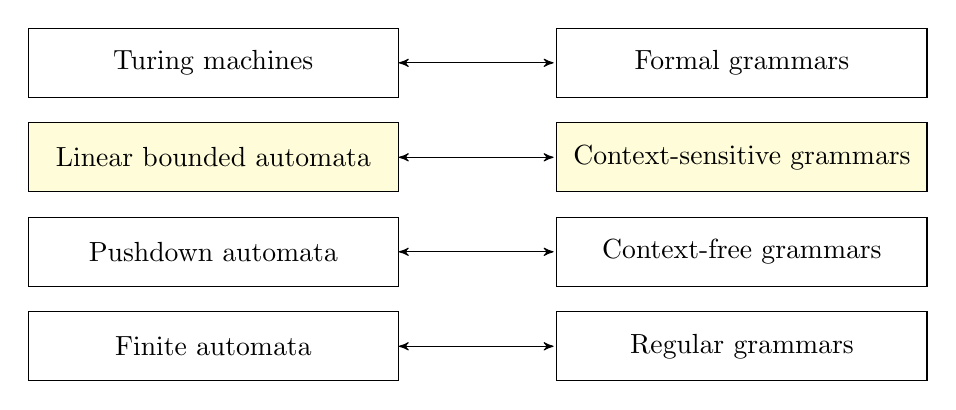
\begin{tikzpicture}[node distance=1.2cm]
        \node[state,rectangle, minimum width =4.7cm][align=center] (fa)      {\alert{Finite automata}};
        \node[state,rectangle, minimum width =4.7cm] (pda) [above of=fa]  {Pushdown automata};
        \node[fill=yellow!15!white,state,rectangle, minimum width =4.7cm] (la) [above of=pda]  {Linear bounded automata};
        \node[state,rectangle, minimum width =4.7cm][align=center] (ts) [above of=la]  {\alert{Turing machines}};
        \node[state,rectangle, minimum width =4.7cm] (rg) [right=2cm of fa]  {Regular grammars};
        \node[state,rectangle, minimum width =4.7cm]  (cfg) [right=2cm of pda]  {\alert{Context-free grammars}};
        \node[fill=yellow!15!white,state,rectangle, minimum width =4.7cm][align=center]  (cg) [above of=cfg]  {Context-sensitive grammars};
        \node[state,rectangle, minimum width =4.7cm] (g0) [above of=cg]  {Formal grammars};
        \path[<->] 
            (fa)  edge node {} (rg)
            (pda)  edge node {} (cfg)
            (la)  edge node {} (cg)
            (ts)  edge node {} (g0)
        ;
    \end{tikzpicture}

    \bigskip

       

\end{frame}


\begin{frame}{Context-sensitive languages}

    \begin{theorem}
        The following are equivalent for a language $L$:
        \begin{enumerate}[(i)]
            \item $L$ is generated by a \alert{context-sensitive} grammar.
            \item $L$ is generated by a \alert{monotone} grammar.
            \item $L$ is recognized by a \alert{Linear Bounded Automaton} (\alert{LBA}).
        \end{enumerate}
    \end{theorem}

    \begin{itemize}
        \item \alert{context-sensitive} grammar: $\alpha_1 A \alpha_2\rightarrow \alpha_1\gamma\alpha_2$ where $A\in V$, $\gamma\in(V\cup T)^+$, $\alpha_1,\alpha_2\in (V\cup T)^*$ ($S\to\epsilon$ if $S$ not in bodies)
        \item \alert{monotone} grammar: $\alpha\to\beta$ where $|\alpha|\leq|\beta|$
        \item \alert{Linear Bounded Automaton} (\alert{LBA}): a nondeterministic TM only using the input portion of the tape [we formalize later]
    \end{itemize}

    \textbf{Note:} Context-sensitive grammars are monotone, $(i)\Rightarrow(ii)$ trivial.\\
    Monotone grammars do not shorten sentential forms in a derivation

\end{frame}


\begin{frame}{Example: $L=\{a^nb^nc^n\mid n\geq 1\} $ is context-sensitive}

    (Recall that $L$ is not context-free.)

    \medskip

    A \alert{monotone} grammar:

    \qquad$S\rightarrow aSBC\mid abC$\hfill{\it right amount of $a,B,C$}\\
    \qquad\alert{$CB\rightarrow BC$}\hfill{\it reorder to $a^nbB^{n-1}C^n$}\\
    \qquad$bB\rightarrow bb$\hfill{\it $B\to b$ only if preceded by $b$}\\
    \qquad$bC\rightarrow bc$\hfill{\it $C\to c$ only if preceded by $b$}\\
    \qquad$cC\rightarrow cc$\hfill{\it\dots or by $c$}

    \bigskip

    The rule $CB\rightarrow BC$ is not context-sensitive. But we can convert it to a chain of context-sensitive rules:

    \qquad$CB\rightarrow XB$, $XB\rightarrow XY$, $XY\rightarrow BY$, $BY\rightarrow BC$

    (Same for any monotone rule, as long as there are no terminals.)
    
\end{frame}


\begin{frame}{From monotone to context-sensitive grammars\hfill $(ii)\Rightarrow(i)$}

    \textbf{Recall:} \alert{separated grammar} means productions of the form $\alpha\rightarrow \beta$ where either $\alpha, \beta\in V^+$ or $\alpha \in V,\beta \in T\cup \{\epsilon\}$

    \begin{lemma}
        Every monotone grammar can be converted to an equivalent context-sensitive grammar.
    \end{lemma}
    \vspace{-6pt}
    \textbf{Proof:}
        First, convert to separated grammar (as for ChNF). This preserves monotonicity, $V_a\to a$ is monotone, context-sensitive.

        Then, convert every production $A_1\ldots A_m\rightarrow B_1\ldots B_n $ ($m\leq n$) to the following chain (using new auxiliary variables $C_i$):
        
        \vspace{-0.9cm}

        \begin{multicols}{2}

            \footnotesize
            
            \begin{align*}
                A_1A_2\ldots A_m & \rightarrow C_1A_2\ldots A_m\\
                C_1A_2\ldots A_m & \rightarrow C_1C_2\ldots A_m\\
                &\ \,\vdots\\
                C_1\ldots C_{m-1}A_m & \rightarrow C_1\ldots C_{m-1} C_m
            \end{align*}

            \newcolumn

            \begin{align*}
                C_1C_2\ldots C_m & \rightarrow B_1C_2\ldots C_m\\
                B_1C_2\ldots C_m & \rightarrow B_1B_2\ldots C_m\\
                &\ \,\vdots\\
                B_1\ldots B_{m-1}C_m & \rightarrow B_1\ldots B_{m-1}B_m\ldots B_n\\                
            \end{align*}
                        
        \end{multicols}

\end{frame}


\begin{frame}{Linear Bounded Automaton}    

    \begin{definition}
        A \alert{linear bounded automaton} (\alert{LBA}) is a \emph{nondeterministic} Turing machine where the tape contains special symbols for left ($\underline{l}$) and right ($\underline{r}$) end. Those symbols cannot be rewritten and the head cannot move to the left of $\underline{l}$ or to the right of $\underline{r}$. 

    A word $w$ is \alert{accepted} if $q_0\underline{l}w\underline{r}\vdash^*\alpha p\beta$ for some $p\in F$
    \end{definition}
    \begin{itemize}
        \item The space for computation is given by the input word, we cannot exceed its length.
        \item Not a problem for context-sensitive/monotone grammars: sentential forms in a derivation cannot shorten.
        \item Nondeterminisim is crucial!
    \end{itemize}

    \alert{Construction trick:} `draw' several tape symbols into one cell (as in multi-track tape), increase space by constant factor; hence `linear'

\end{frame}


\begin{frame}{From monotone grammar to LBA \hfill $(ii)\Rightarrow(iii)$}

    \begin{columns}

        \column{0.62\textwidth}

        %Split the tape into two tracks:

        \alert{Track 1}: a copy of the input $w$, read-only

        \alert{Track 2}: simulate the derivation of $w$ %(monotone $\Rightarrow$ it fits below $w$)
        
        \column{0.38\textwidth}
    
        \vspace{11pt}

        \scalebox{0.9}{
            \begin{tabular}{|c| c c |c|}
                \hline
                \multirow{2}{*}{\underline{l}} & \multicolumn{2}{c|}{w}& \multirow{2}{*}{\underline{r}}\\ \cline{2-3}
                & \multicolumn{1}{c|}{S}& \hspace{2cm} &\\\hline
            \end{tabular}                
        }

        
    \end{columns}

    \begin{itemize}
        \item initialize with $S$ in first field (the rest blank)
        \item at the end it should contain $w$, compare to Track 1  
        
        \bigskip
        
        \item to simulate one derivation step (apply rule $\alpha X \beta \rightarrow \alpha \gamma \beta$):

        \smallskip
        \begin{center}
            \begin{tabular}{c c c  c c c}
            \cline{1-5}
            \multicolumn{1}{|c|}{u} & $\alpha$ & \multicolumn{1}{|c|}{X} & $\beta$& \multicolumn{1}{|c|}{v} &\\ \cline{1-5}
            \vspace{0.005cm}\\ \cline{1-6}
            \multicolumn{1}{|c|}{u} & $\alpha$ & \multicolumn{2}{|c|}{$\gamma$} & $\beta$& \multicolumn{1}{|c|}{v} \\ \cline{1-6}
            \end{tabular}
        \end{center}
        \smallskip
    
        \item rewrite the sentential form using production rules
        \item \alert{nondeterministically choose} which rule and where to apply it
        \item rewrite head to body (move the rest to the right)
        \item if only terminals, compare with Track 1, accept if match\hfill\qedsymbol
    \end{itemize}

\end{frame}


\begin{frame}{From LBA to monotone grammar}
    
    \begin{itemize}
        \item the grammar cannot generate any `extra' symbols
        \item we hide the computation in `two-track' variables
        \item generate a word of the form $$(a_0,\left[q_0,\underline{l},a_0\right]),(a_1,a_1),\ldots,(a_n,\left[a_n,\underline{r}\right]) $$

        \medskip

        \begin{center}
            \begin{tabular}{|c c c|}
            \hline
            \multicolumn{3}{|c|}{w} \\ \cline{1-3}
            \multicolumn{1}{|c|}{$q_0,\underline{l},a_0$}& \hspace{2cm} &\multicolumn{1}{|c|}{$a_n,\underline{r}$}\\\hline
            \end{tabular}
        \end{center}

        \bigskip
        
        \item simulate computation in the 2nd track (as for TMs)
        \begin{itemize}
            \item for $\delta(p,x)\ni(q,x',R)$:  $P\underline{X}\underline{Y}\rightarrow \underline{X'}Q\underline{Y}$ 
            \item for $\delta(p,x)\ni(q,x',L)$:  $\underline{Y}P\underline{X}\rightarrow Q\underline{Y}\underline{X'} $ 
        \end{itemize}
    \item if the state is accepting, `erase' the 2nd track
    \item special production for generating $\epsilon$ (if $\epsilon \in L$)\hfill\qedsymbol
    \end{itemize}

\end{frame}


% TODO: Add an example of the construction?


\begin{frame}{Hierarchy of languages: context-sensitive and above}
    
    \small\vspace{-10pt}
    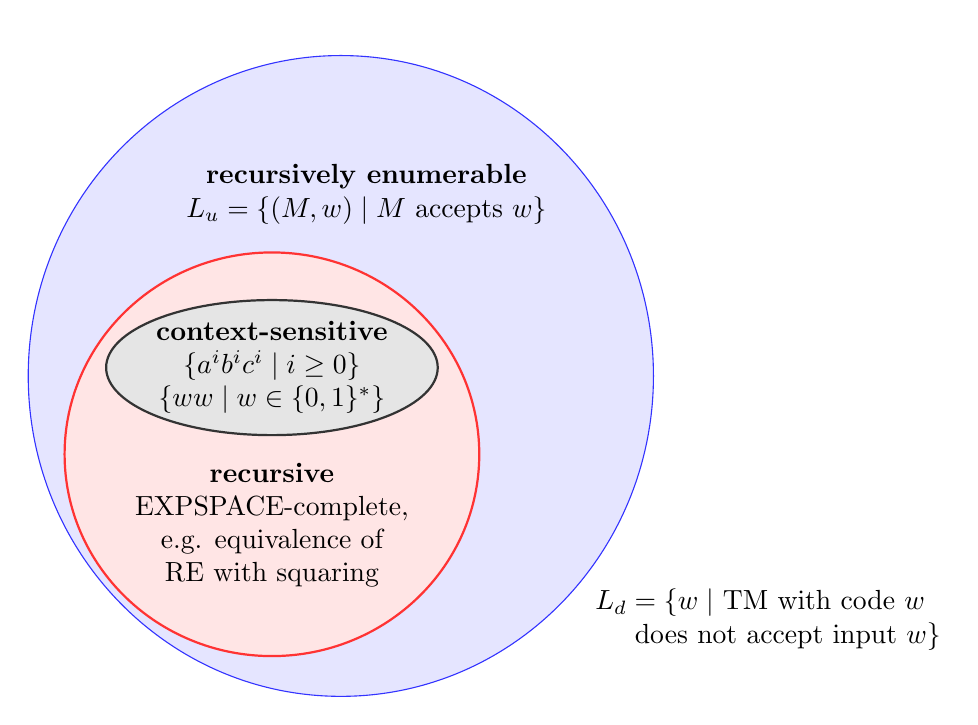
\begin{tikzpicture}[level distance=8mm]
        \node[align=center] (rr) at (1,0) {\textbf{recursive}\\ EXPSPACE-complete, \\e.g. equivalence of\\ RE with squaring};
        % example: equivalence of regular expressions with squaring
        \node[align=center] (cl) at (1,2) {\textbf{context-sensitive}\\$\{a^ib^ic^i\mid i\geq 0\} $\\$\{ww\mid w\in \{0,1\}^*\} $};
        \node[align=center] (re) at (2.2,4.2) {\textbf{recursively enumerable}\\$L_u=\{(M,w)\mid M\text{ accepts }w\}$};
        \node[align=center] (out) at (7.2,-1.2) {$L_d=\{w\mid$ TM with code $w$\\ \qquad does not accept input $w\}$};
        \node (bot) at (1,-1.2) {};
        \node (top) at (1,6.2) {};
        \node (left) at (-1.2,0) {};
        
        \node[draw=blue!80,inner sep=2pt,ellipse,fit=(rr) (cl) (re)] {};
        \node[draw=red!80,thick,inner sep=0pt,ellipse,fit=(rr) (cl)] {};
        \node[draw=black!80,thick,inner sep=-3pt,ellipse,fit= (cl)] {};
        
        \begin{scope}[on background layer]
            \node[fill=blue!10,inner sep=2pt,ellipse,fit=(rr) (cl) (re)] {};
            \node[fill=red!10,thick,inner sep=0pt,ellipse,fit=(rr) (cl)] {};
            \node[fill=black!10,thick,inner sep=-3pt,ellipse,fit= (cl)] {};
        \end{scope}
    \end{tikzpicture}
    
\end{frame}


\section{\sc Chapter 4: Intro to computability theory}


\section*{First, a brief overview in 4 slides, without technical details}


\begin{frame}{Languages and decision problems}
    
    A \alert{decision problem} $P$: given input $w$ (usually a 0-1 string), answer YES or NO (e.g. `Is the given number prime?',  `Is the given picture classified as cat by the given neural net?')
    
    \vspace{-10pt}
    $$
    \alert{L_P}=\{w\mid P(w)\text{ answers `YES'}\}
    $$

    \begin{itemize}
        \item $P$ is \alert{(algorithmically) decidable} $\Leftrightarrow$ $L_P$ is \alert{recursive} $\Leftrightarrow$ there is a TM \alert{deciding} $L_P$ (halting on every input, answering correctly)
        \item $P$ is \alert{partially decidable} $\Leftrightarrow$ $L_P$ is \alert{recursively enumerable} $\Leftrightarrow$ there is a TM that accepts every YES-instance $w$ but for NO-instances it may either reject or run an infinite loop
    \end{itemize}

    \textbf{NB:} almost all problems are not even partially decidable (TMs can be represented by finite strings, so only countably many TMs)
    
    \textbf{Coming up next:} a concrete example, the \alert{diagonal language}

\end{frame}


\begin{frame}{Source code for a Turing Machine \& how to execute it}

    Source code for TMs:
    \begin{itemize}
        \item encode TMs by 01-strings, $M\ \rightsquigarrow\ \alert{\mathrm{code}(M)}\in\{0,1\}^*$
        \item if $w$ is not well-formed code, then say it represents a TM with no transitions, so every $w\in\{0,1\}^*$ will represent some TM
        \item also encode a pair of 01-strings $u,v$ as a 01-string $\langle u,v\rangle$
    \end{itemize}

    \medskip

    The \alert{Universal language}: $L_U=\{\langle \mathrm{code(M),w}\rangle\mid M\text{ accepts }w\}$

    \medskip
    
    \begin{quote}
        ``Does a given program return true on a given input?''
    \end{quote}

    \medskip

    \begin{theorem}
        The Universal language is recursively enumerable.
    \end{theorem}

    \textbf{Proof idea:} construct the \alert{Universal Turing Machine} that can simulate any TM (using its code) on any input [details later]

\end{frame}


\begin{frame}{Barber's paradox aka the diagonal argument}


    The \alert{Diagonal language}:
    $$
    L_D=\{w\mid M\text{ such that $w=\mathrm{code}(M)$ does *not* accept }w\}
    $$

    \medskip
    
    \begin{quote}
        ``Return true if the given program does not return true when fed its own source code.''
    \end{quote}

    \medskip

    \begin{theorem}
        The Diagonal language is not recursively enumerable.
    \end{theorem}

    \textbf{Proof idea:} there cannot exist a TM recognizing $L_
    D$: running it on its own code would lead to Barber's paradox

    \bigskip

    \begin{quote}
        ``The program accepts all programs that don't accept themselves. Does the program accept itself?''
    \end{quote}    

\end{frame}


\begin{frame}{Languages that are recursively enumerable, but not recursive}

    \begin{block}{Post's theorem}
        A language $L$ is recursive, if and only if both $L$ and $\overline{L}$ are recursively enumerable.
    \end{block}
    
    \vspace{-6pt}
    \textbf{Proof idea:} simulate TMs for $L$ and $\overline{L}$ in parallel, one must halt
    \vspace{6pt}

    \begin{corollary}
        The language $\overline{L_D}$ is not recursive, but it is recursively enumerable.
    \end{corollary}

    \vspace{-6pt}
    {\it ``Does the given program return true when fed its own code?''}
    \vspace{6pt}

    \begin{corollary}
        The Universal language is not recursive.
    \end{corollary}
    
    \vspace{-6pt}
    (If a TM decided $L_U$, we could use it to decide $\overline{L_D}$: $w\rightsquigarrow\langle w,w\rangle$)
    \vspace{9pt}

    We can execute a program, but cannot test if it runs into a loop.    

\end{frame}


\section*{Now, the technical details}


\begin{frame}{Machine-readable encoding of TMs (Gödel numbering)}

    \vspace{-5pt}
    To encode a TM as a binary string, we first assign integers to the states, tape symbols, and directions $L,R$. Assume:
    \begin{itemize}
        \item the start state is always $q_1$, the only final state is $q_2$
        \item the first tape symbol is always 0, the second 1, the third B (other tape symbols can be assigned arbitrarily)
        \item the direction L is 1, the direction R is 2
    \end{itemize}
    Each transition $\delta(q_i,X_j)=(q_k,X_l,D_m)$ is encoded by $0^i10^j10^k10^l10^m$. Since $i,j,k,l,m\geq 1$, substring 11 doesn't occur.
    The entire encoding \alert{$\mathrm{code}(M)$} consists of codes for all transitions (in any order), separated by a pair of 1's: $C_111C_211\ldots C_{n-1}11C_n$.

    Similarly, we can encode a tuple of 01-strings as a 01-string. We also fix an order of 01-strings, by length + lexicographically \\ ($w_0=\epsilon$, $w_1=0$, $w_2=1$, $w_3=00$, $w_4=01$, \dots)

\end{frame}


\begin{frame}{Example}

    $$
    M=(\{q_1,q_2,q_3\},\{0,1\},\{0,1,B\},\delta,q_1,B,\{q_2\})
    $$

    \begin{center}
        \begin{tabular}{r |c |c |c }
        $\delta$ & 0 & 1 & B \\
        \hline\hline
        $\rightarrow q_1$& & $(q_3,0,R)$& \\
        $*q_2$& & & \\
        $q_3$& $(q_1,1,R)$&$(q_2,0,R)$ &$(q_3,1,L)$.
        \end{tabular}
    \end{center}

    Codes for transitions:
    \vspace{-12pt}
    \begin{center}
        \small
        \begin{tabular}{c|c|c|c}
            $C_1$&$C_2$&$C_3$&$C_4$\\
            0100100010100&
            0001010100100&
            00010010010100&
            0001000100010010
        \end{tabular}
    \end{center} 
    
    \medskip
    
    The full encoding $\mathrm{code}(M)$:
    \vspace{-12pt}
    \begin{center}
        \small
        $$
        01001000101001100010101001001100010010010100110001000100010010
        $$        
    \end{center}

\end{frame}


\begin{frame}{Summary of Lecture 11}

    \begin{itemize}        
        \item Recursively enumerable languages are exactly those generated by (Type 0) grammars
        \begin{itemize}
            \item TM to G: simulate moves on a reversed non-terminal copy of $\omega$, generate sufficient space, cleanup if accepting state
            \item G to TM: generate all strings, check if any of them represents a valid derivation of $\omega$ (sentential forms separated by $\#$)
        \end{itemize}   
        \item Context-sensitive languages:
        \begin{itemize}
            \item context-sensitive grammars are equivalent to monotone grammars
            \item Linear Bounded Automaton (LBA): nondeterministic TM with tape limited to the length of input
            \item constructions: monotone grammar to LBA, LBA to monotone grammar
        \end{itemize}
        \item Intro to computability: an overview
        \item decision problem $\leftrightsquigarrow$ the language of all `YES' instances
        \item machine-readable encoding of TMs
    \end{itemize}
    
\end{frame}









\end{document}




